% Options for packages loaded elsewhere
\PassOptionsToPackage{unicode}{hyperref}
\PassOptionsToPackage{hyphens}{url}
%
\documentclass[
]{article}
\title{Tidyverse Learnings}
\author{Can Aytöre}
\date{2022-02-17}

\usepackage{amsmath,amssymb}
\usepackage{lmodern}
\usepackage{iftex}
\ifPDFTeX
  \usepackage[T1]{fontenc}
  \usepackage[utf8]{inputenc}
  \usepackage{textcomp} % provide euro and other symbols
\else % if luatex or xetex
  \usepackage{unicode-math}
  \defaultfontfeatures{Scale=MatchLowercase}
  \defaultfontfeatures[\rmfamily]{Ligatures=TeX,Scale=1}
\fi
% Use upquote if available, for straight quotes in verbatim environments
\IfFileExists{upquote.sty}{\usepackage{upquote}}{}
\IfFileExists{microtype.sty}{% use microtype if available
  \usepackage[]{microtype}
  \UseMicrotypeSet[protrusion]{basicmath} % disable protrusion for tt fonts
}{}
\makeatletter
\@ifundefined{KOMAClassName}{% if non-KOMA class
  \IfFileExists{parskip.sty}{%
    \usepackage{parskip}
  }{% else
    \setlength{\parindent}{0pt}
    \setlength{\parskip}{6pt plus 2pt minus 1pt}}
}{% if KOMA class
  \KOMAoptions{parskip=half}}
\makeatother
\usepackage{xcolor}
\IfFileExists{xurl.sty}{\usepackage{xurl}}{} % add URL line breaks if available
\IfFileExists{bookmark.sty}{\usepackage{bookmark}}{\usepackage{hyperref}}
\hypersetup{
  pdftitle={Tidyverse Learnings},
  pdfauthor={Can Aytöre},
  hidelinks,
  pdfcreator={LaTeX via pandoc}}
\urlstyle{same} % disable monospaced font for URLs
\usepackage[margin=1in]{geometry}
\usepackage{color}
\usepackage{fancyvrb}
\newcommand{\VerbBar}{|}
\newcommand{\VERB}{\Verb[commandchars=\\\{\}]}
\DefineVerbatimEnvironment{Highlighting}{Verbatim}{commandchars=\\\{\}}
% Add ',fontsize=\small' for more characters per line
\usepackage{framed}
\definecolor{shadecolor}{RGB}{248,248,248}
\newenvironment{Shaded}{\begin{snugshade}}{\end{snugshade}}
\newcommand{\AlertTok}[1]{\textcolor[rgb]{0.94,0.16,0.16}{#1}}
\newcommand{\AnnotationTok}[1]{\textcolor[rgb]{0.56,0.35,0.01}{\textbf{\textit{#1}}}}
\newcommand{\AttributeTok}[1]{\textcolor[rgb]{0.77,0.63,0.00}{#1}}
\newcommand{\BaseNTok}[1]{\textcolor[rgb]{0.00,0.00,0.81}{#1}}
\newcommand{\BuiltInTok}[1]{#1}
\newcommand{\CharTok}[1]{\textcolor[rgb]{0.31,0.60,0.02}{#1}}
\newcommand{\CommentTok}[1]{\textcolor[rgb]{0.56,0.35,0.01}{\textit{#1}}}
\newcommand{\CommentVarTok}[1]{\textcolor[rgb]{0.56,0.35,0.01}{\textbf{\textit{#1}}}}
\newcommand{\ConstantTok}[1]{\textcolor[rgb]{0.00,0.00,0.00}{#1}}
\newcommand{\ControlFlowTok}[1]{\textcolor[rgb]{0.13,0.29,0.53}{\textbf{#1}}}
\newcommand{\DataTypeTok}[1]{\textcolor[rgb]{0.13,0.29,0.53}{#1}}
\newcommand{\DecValTok}[1]{\textcolor[rgb]{0.00,0.00,0.81}{#1}}
\newcommand{\DocumentationTok}[1]{\textcolor[rgb]{0.56,0.35,0.01}{\textbf{\textit{#1}}}}
\newcommand{\ErrorTok}[1]{\textcolor[rgb]{0.64,0.00,0.00}{\textbf{#1}}}
\newcommand{\ExtensionTok}[1]{#1}
\newcommand{\FloatTok}[1]{\textcolor[rgb]{0.00,0.00,0.81}{#1}}
\newcommand{\FunctionTok}[1]{\textcolor[rgb]{0.00,0.00,0.00}{#1}}
\newcommand{\ImportTok}[1]{#1}
\newcommand{\InformationTok}[1]{\textcolor[rgb]{0.56,0.35,0.01}{\textbf{\textit{#1}}}}
\newcommand{\KeywordTok}[1]{\textcolor[rgb]{0.13,0.29,0.53}{\textbf{#1}}}
\newcommand{\NormalTok}[1]{#1}
\newcommand{\OperatorTok}[1]{\textcolor[rgb]{0.81,0.36,0.00}{\textbf{#1}}}
\newcommand{\OtherTok}[1]{\textcolor[rgb]{0.56,0.35,0.01}{#1}}
\newcommand{\PreprocessorTok}[1]{\textcolor[rgb]{0.56,0.35,0.01}{\textit{#1}}}
\newcommand{\RegionMarkerTok}[1]{#1}
\newcommand{\SpecialCharTok}[1]{\textcolor[rgb]{0.00,0.00,0.00}{#1}}
\newcommand{\SpecialStringTok}[1]{\textcolor[rgb]{0.31,0.60,0.02}{#1}}
\newcommand{\StringTok}[1]{\textcolor[rgb]{0.31,0.60,0.02}{#1}}
\newcommand{\VariableTok}[1]{\textcolor[rgb]{0.00,0.00,0.00}{#1}}
\newcommand{\VerbatimStringTok}[1]{\textcolor[rgb]{0.31,0.60,0.02}{#1}}
\newcommand{\WarningTok}[1]{\textcolor[rgb]{0.56,0.35,0.01}{\textbf{\textit{#1}}}}
\usepackage{longtable,booktabs,array}
\usepackage{calc} % for calculating minipage widths
% Correct order of tables after \paragraph or \subparagraph
\usepackage{etoolbox}
\makeatletter
\patchcmd\longtable{\par}{\if@noskipsec\mbox{}\fi\par}{}{}
\makeatother
% Allow footnotes in longtable head/foot
\IfFileExists{footnotehyper.sty}{\usepackage{footnotehyper}}{\usepackage{footnote}}
\makesavenoteenv{longtable}
\usepackage{graphicx}
\makeatletter
\def\maxwidth{\ifdim\Gin@nat@width>\linewidth\linewidth\else\Gin@nat@width\fi}
\def\maxheight{\ifdim\Gin@nat@height>\textheight\textheight\else\Gin@nat@height\fi}
\makeatother
% Scale images if necessary, so that they will not overflow the page
% margins by default, and it is still possible to overwrite the defaults
% using explicit options in \includegraphics[width, height, ...]{}
\setkeys{Gin}{width=\maxwidth,height=\maxheight,keepaspectratio}
% Set default figure placement to htbp
\makeatletter
\def\fps@figure{htbp}
\makeatother
\setlength{\emergencystretch}{3em} % prevent overfull lines
\providecommand{\tightlist}{%
  \setlength{\itemsep}{0pt}\setlength{\parskip}{0pt}}
\setcounter{secnumdepth}{5}
\ifLuaTeX
  \usepackage{selnolig}  % disable illegal ligatures
\fi
\usepackage[]{natbib}
\bibliographystyle{plainnat}

\begin{document}
\maketitle

{
\setcounter{tocdepth}{2}
\tableofcontents
}
\hypertarget{the-r-language}{%
\section{The R Language}\label{the-r-language}}

The R language is an extremely popular scripting language used by millions of people around the world. Primarily, it's used for data analysis, modeling, and visualization. Many people think of R as statistical software, but it's fundamentally not and it's a little bit upsetting when people say that. R is programming language that has been adopted and curated by people interested in doing data science as flexibly as possible.

R lives and breathes at the comprehensive R archive network, abbreviated to CRAN. When you download R from CRAN, you've actually installed Base-R. Base-R includes all of the necessary machinery for your computer to be able to run R code. It also installs standard R packages like \texttt{stats}, \texttt{utils} and \texttt{graphics}. These packages allow you to start using R immediately on your machine. In order for data manipulation, using Base R is sufficient most of the time. The Base R way of doing things involves a code that looks very much like this;

\begin{Shaded}
\begin{Highlighting}[]
\FunctionTok{head}\NormalTok{(iris[iris}\SpecialCharTok{$}\NormalTok{Species }\SpecialCharTok{==} \StringTok{"virginica"}\NormalTok{,])}
\end{Highlighting}
\end{Shaded}

\begin{verbatim}
##     Sepal.Length Sepal.Width Petal.Length Petal.Width   Species
## 101          6.3         3.3          6.0         2.5 virginica
## 102          5.8         2.7          5.1         1.9 virginica
## 103          7.1         3.0          5.9         2.1 virginica
## 104          6.3         2.9          5.6         1.8 virginica
## 105          6.5         3.0          5.8         2.2 virginica
## 106          7.6         3.0          6.6         2.1 virginica
\end{verbatim}

First to access to `species' column and then we have a double equals to say `species' is equivalent to `virginica' and then we have a comma to say we want all of the columns and then the final closing square bracket.

\hypertarget{r-packages}{%
\subsection{R Packages}\label{r-packages}}

It's possible to do every single thing you could possibly imagine with Base-R because it is a true and complete programming language but you would have to write a lot of code yourself. Most people jump straight into using R packages to make their life easier and more reproducible, so what are R packages? R packages are self-contained collections of functions and/or datasets that provide us with the ability to do any number of things from analyzing data, visualizing data to potentially even generating reports with R which is what R Markdown allows us to do. Now, CRAN has over 10,000 packages and this comprehensive range of packages available from CRAN is part of what makes R such a popular scripting language.

It's a fact of programming and scripting but building everything yourself from scratch is time consuming and more than likely, hugely error prone, this is why R users depend on packages. Using packages makes it easier to start working on a new project in R. Packages can make collaborating with others on R projects easier, as you can be ensured everyone is using the same code base.

\hypertarget{what-is-tidyverse}{%
\section{What is Tidyverse?}\label{what-is-tidyverse}}

There are definitely one or two packages that would make your life with R a little bit easier, i.e.~they're designed to do the kind of analysis or data visualization which is important to your domain-specific knowledge. The tidyverse is an ecosystem of R packages designed to work consistently and interdependently together to provide a flexible and easy-to-understand workflow for doing data science with the R language. The fundamental building block of the tidyverse is the concept of tidy data. The tidyverse has been in development since early 2014 and is becoming increasingly mature. But the tidyverse should never be considered a replacement for Base R. It will remain crucial to understand the base R way of doing things.

\begin{itemize}
\tightlist
\item
  In other words, the tidyverse is both a collection of R packages, and an approach to how to do data science effectively, and reproducibly with the R language.
\end{itemize}

\hypertarget{why-use-the-tidyverse}{%
\subsection{Why use the Tidyverse?}\label{why-use-the-tidyverse}}

So what makes the tidyverse different? Well, the core of the tidyverse is developed by developers at RStudio. It's a company with an extremely good reputation including, for R package development. RStudio's own internal tools dependent on components of the tidyverse, helping to reassure us of the long term viability of the tidyverse ecosystem. Tidyverse is developed openly on GitHub, meaning users can track continuing development and if necessary, fork packages in the future if Rstudio themselves, stop updating them.

\hypertarget{strengths-of-tidyverse}{%
\subsection{Strengths of Tidyverse}\label{strengths-of-tidyverse}}

What does the tidyverse provide us as end users or data scientists? Well, using tidyverse leads to advantages in the following main areas:
- Data importation
- Data wrangling
- Data visualization

\hypertarget{data-import}{%
\subsubsection{Data import}\label{data-import}}

Let's look at each of those. \texttt{readr} completely blows away the base-R tools for importing rectangular data files like csv (comma-separated values) and tsv (tab-separated values) files. It's not only significantly faster than base-R but it's more intelligent. For instance, automatically converting dates to dates, times to times, and converting columns that should be numbers into numbers. And finally, it never ever imports columns of strings as factors. If you're already a base-R user, chances are you've spent hours of frustration because of this issue using base-R. \textbf{This section} includes importing data with \texttt{readr} as it's for general workhorse of most R users data import toolkit. The \texttt{readxl} library makes importing from excel files ridiculously simple allowing worksheets, individual cells, or even cell ranges to be targeted for import easily. The tidyverse also aims to fit into existing workflows. \texttt{haven} allows data to be imported from SAS, SPSS, and Stata. Now these three packages significantly decrease the time needed to massage data files into R. And help solve a number of common frustrations with base-R packages. But please note that \texttt{readr} is the only package of the three that is part of the core \texttt{tidyverse}. You need to separately load \texttt{readxl} and \texttt{haven} to access those libraries.

\hypertarget{data-wrangling}{%
\subsubsection{Data wrangling}\label{data-wrangling}}

The tidyverse utilizes the pipe operator (\%\textgreater\%). This percentage greater than percentage thing to provide a logical framework for chaining together common data wrangling tasks. This makes code very faster to write and easier to read. There's \textbf{a chapter} dedicated to the pipe operator as it is mysterious magic to many R users. The tidyverse is designed around a concept of \emph{tidydata}. The \texttt{tidyr} library is designed for reshaping and transforming your imported data into a structure ready to manipulate, model, and visualize with the tidyverse. \texttt{dplyr} is the library for sub-setting, filtering, summarizing, and generally wrangling your data. It also provides a number of tools for doing database-like operations for working on relational datasets. These packages used together form a core data processing component of the tidyverse. The operations you'll perform with these are both significantly faster and simpler to construct than simply using base-R. \texttt{ggplot2} provides a complete consistent and incredibly powerful grammar of graphics, allowing impressive static visualizations to be built with minimal effort.

I'm going to quickly show what's possible using all the components for tidyverse together. After loading libraries \texttt{gapminder} and \texttt{tidyverse}, we have a little bit of code which uses \texttt{dplyr} (to group my data by continent and year, and then summaries to calculate the continent population). And then I use \texttt{ggplot2} to generate my chart. I have quite a beautiful looking \textbf{static} visualization generated with \texttt{ggplot2}. It's important to know that \texttt{ggplot2} provides a powerful consistent grammar for creating static shots.

\begin{Shaded}
\begin{Highlighting}[]
\FunctionTok{library}\NormalTok{(}\StringTok{"gapminder"}\NormalTok{)}
\FunctionTok{library}\NormalTok{(}\StringTok{"tidyverse"}\NormalTok{)}

\NormalTok{gapminder }\SpecialCharTok{\%\textgreater{}\%}
  \FunctionTok{group\_by}\NormalTok{(continent, year) }\SpecialCharTok{\%\textgreater{}\%}
  \FunctionTok{summarise}\NormalTok{(}\AttributeTok{continent.population =} \FunctionTok{sum}\NormalTok{(}\FunctionTok{as.numeric}\NormalTok{(pop))) }\SpecialCharTok{\%\textgreater{}\%}
  \FunctionTok{ggplot}\NormalTok{(}\FunctionTok{aes}\NormalTok{(}\AttributeTok{x =}\NormalTok{ year, }\AttributeTok{y =}\NormalTok{ continent.population)) }\SpecialCharTok{+}
  \FunctionTok{geom\_area}\NormalTok{(}\FunctionTok{aes}\NormalTok{(}\AttributeTok{fill =}\NormalTok{ continent), }\AttributeTok{position =} \StringTok{"stack"}\NormalTok{) }\SpecialCharTok{+}
  \FunctionTok{ggtitle}\NormalTok{(}\StringTok{"Gapminder population growth per continent"}\NormalTok{,}
          \AttributeTok{subtitle =} \FunctionTok{paste}\NormalTok{(}\StringTok{"from"}\NormalTok{, }\FunctionTok{min}\NormalTok{(gapminder}\SpecialCharTok{$}\NormalTok{year), }\StringTok{"to"}\NormalTok{, }\FunctionTok{max}\NormalTok{(gapminder}\SpecialCharTok{$}\NormalTok{year)))}
\end{Highlighting}
\end{Shaded}

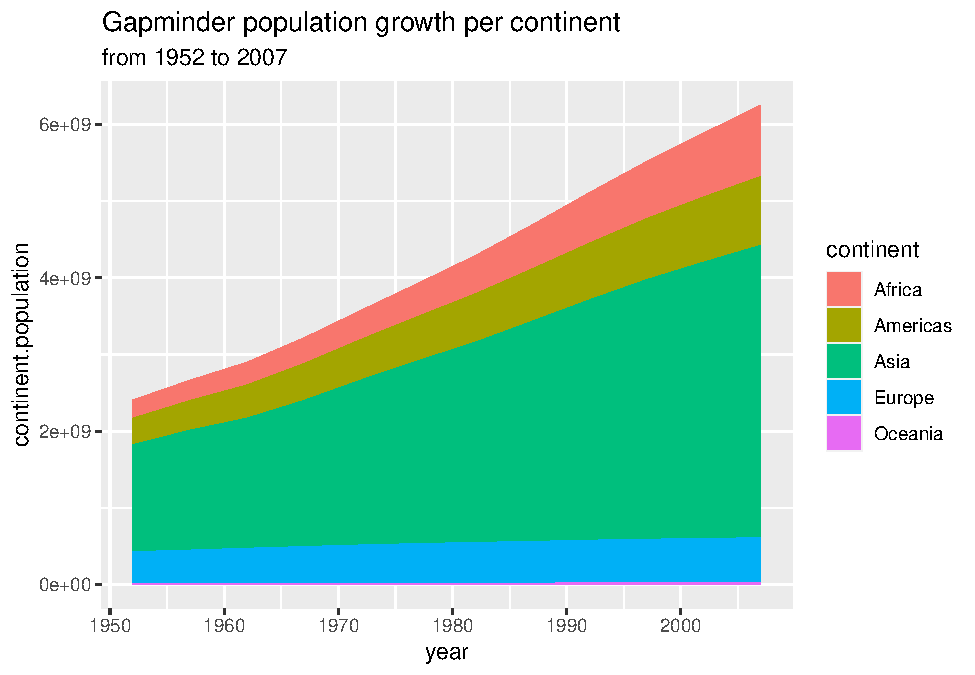
\includegraphics{tidyverse_learnings_files/figure-latex/unnamed-chunk-2-1.pdf}

If you're interested in building interactive charts for the web with R, you'll need to learn about \texttt{htmlwidgets}. But in most commonly used \texttt{htmlwidgets} libraries, lean heavily on the tidyverse for preparing data for visualization. Plus all the good \texttt{htmlwidgets} are designed to use the pipe operator. Let's have a look at what we could build using \texttt{htmlwidgets} in R. We use the \texttt{dplyr} library to wrangler our data. And then we build our chart in the \texttt{highcharter} library. So instead of a \textbf{static} chart, what we have now is an \textbf{interactive} chart that I can move my cursor through and get information for specific points in the dataset. I can also actually remove series if I'm interested in doing that. So, \texttt{ggplot2} is part of the \texttt{tidyverse} and allows us to build static charts in a consistent manner. \texttt{htmlwidgets} allows us to create interactive charts and often depends on the tidyverse for wrangling and constructing our data for visualization.

\begin{Shaded}
\begin{Highlighting}[]
\FunctionTok{library}\NormalTok{(}\StringTok{"gapminder"}\NormalTok{)}
\FunctionTok{library}\NormalTok{(}\StringTok{"tidyverse"}\NormalTok{)}
\FunctionTok{library}\NormalTok{(}\StringTok{"highcharter"}\NormalTok{)}

\NormalTok{gapminder }\SpecialCharTok{\%\textgreater{}\%}
  \FunctionTok{group\_by}\NormalTok{(continent, year) }\SpecialCharTok{\%\textgreater{}\%}
  \FunctionTok{summarise}\NormalTok{(}\AttributeTok{continent.population =} \FunctionTok{sum}\NormalTok{(}\FunctionTok{as.numeric}\NormalTok{(pop))) }\SpecialCharTok{\%\textgreater{}\%}
  \FunctionTok{hchart}\NormalTok{(}\StringTok{"area"}\NormalTok{,}
         \FunctionTok{hcaes}\NormalTok{(}\AttributeTok{x =}\NormalTok{ year, }
               \AttributeTok{y =}\NormalTok{ continent.population, }
               \AttributeTok{group =}\NormalTok{ continent)}
\NormalTok{         ) }\SpecialCharTok{\%\textgreater{}\%}
  \FunctionTok{hc\_plotOptions}\NormalTok{(}\AttributeTok{area =} \FunctionTok{list}\NormalTok{(}\AttributeTok{stacking =} \StringTok{"normal"}\NormalTok{)) }\SpecialCharTok{\%\textgreater{}\%}
  \FunctionTok{hc\_tooltip}\NormalTok{(}\AttributeTok{shared =} \ConstantTok{TRUE}\NormalTok{)}
\end{Highlighting}
\end{Shaded}

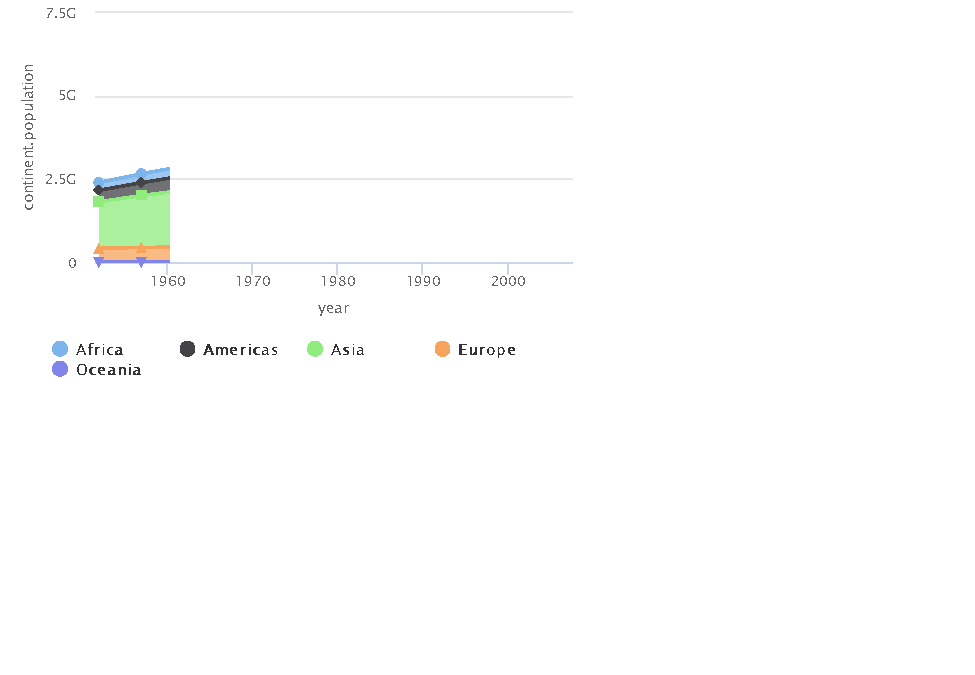
\includegraphics{tidyverse_learnings_files/figure-latex/unnamed-chunk-3-1.pdf}

And finally, there's the \texttt{shiny} library which allows us to build web applications using only the R language without knowing any html or javascript. And \texttt{shiny} allows us to use \texttt{htmlwidgets} to embed interactive charts inside of our web applications.

\hypertarget{maintain-the-tidyverse}{%
\subsection{Maintain the Tidyverse}\label{maintain-the-tidyverse}}

So how do we go about maintaining the tidyverse? Well, remember that in order to use the tidyverse on our system we've installed three discrete things: R itself, RStudio, and the tidyverse collection of packages. To keep fully up to date with the tidyverse, unfortunately we really need to keep on top of all three of these things individually. So let's look at how we do that.

The process you need to go through to keep up to date with R is the most frustrating of all the three tools since there's not a consistent way to do this from within RStudio. Base-R is updated approximately 4 times a year but there's not a regular release cycle. I'd advise that you check every few months for a new version of R. If R console tells you there's a newer version then type a y + Enter and this will launch you to your web browser to the downloads page for R for your operating system. When you're there it's really important to check the release date of that version of R. I thoroughly advise that you do not update R until the release is at least one month old. This is to give the package maintainers that you rely on enough time to update their packages to depend on this new version of R.

So how about updating RStudio? Well, RStudio will automatically check whether there's a new version of RStudio available when you open it up. Updates are typically released a few times a year and generally they include awesome new features that are of general interest. For instance support for new features in R markdown documents or simply making it easier to publish Shiny apps. I thoroughly recommend that as soon as RStudio tells you there's a new version click update, it will take you to the RStudio website and allow you to download the new version.

So how about keeping the tidyverse up to date? Well thankfully that's quite simple. The constituent components of the tidyverse don't have a regular update frequency but that doesn't matter as we have the wonderful tidyverse update function which handles everything for us.

\begin{Shaded}
\begin{Highlighting}[]
\FunctionTok{tidyverse\_update}\NormalTok{()}
\end{Highlighting}
\end{Shaded}

In RStudio simply run the function tidyverse update, it will go away and check are there new versions or packages available, and if so it will grab those versions and install them ready for you to use. Now you might sometimes hear on the grapevine that there are new features available in the development versions of the tidyverse packages. So where do these development versions live? Well they all live on GitHub and you can install the development version of a tidyverse library using the dev tools library if necessary. But where is this grapevine of news about tidyverse? Well one of the best places to keep up to date with what's going on in the tidyverse, and in R in general, is on Twitter. The core RStudio development team are actually very active here and the two hashtags that you want to look out for are rstats and tidyverse. So if you do want one of these development builds of a tidyverse package, as I mentioned, you use the dev tools library and the function install github. But how about if you find that the development version isn't just working out for you, you want to return to the stable version? Well at any time simply use the function install.packages tidyverse and this will recover you to the crown version of all the libraries within the tidyverse.

\hypertarget{references}{%
\subsection{References}\label{references}}

\end{document}
